\section{\texorpdfstring{$\lambda$}{lambda}演算}

\subsection{\texorpdfstring{$\lambda$}{lambda}演算简介}
\subsubsection{从外延的和内涵的角度考虑函数}
现代数学中, \textbf{\textit{函数}}往往被认为是一种\textbf{图的概念} (functions as graphs)\cite{vladimira.zorichMathematicalAnalysis2015}. 也就是说, 对于给定的定义域$X$和陪域$Y$, 函数$f:X\to Y$有如下的定义
\[
    f:=\{(x, y)\in X\times Y\mid \forall x\in X(\exists!y\in Y(f(x)=y))\}
\]
定义在 $X$上的两个函数$f:X\to Y$和$g:X\to Y$被认为是\textit{\textbf{相等的}}当且仅当
\[
    \forall x\in X(f(x)=g(x))    
\]
这样的观点被认为是从外延的 (extensionally) 角度看待函数, 因为基于这样的观点, 人们并不关心函数内部是如何工作的, 他们只关心函数映射的结果如何. 

但是在20世纪之前, 人们更多地把函数看作一种\textbf{规则的概念} (functions as rules). 因为那时人们更关注的是函数如何计算的: 确定一个函数, 你应该要确定它的表达式. 比如说, 
\[
    f(x)=\sin(x^2)  \quad x\in \mathbb R  
\]
就被认为是一个典型的函数.和上面的观点相对应地, 这样的观点被认为是从\textbf{\textit{内涵}} (intensionally) 的角度考察函数.

显然对于大部分数学家来说, 将函数看作是\textbf{图的概念}要更加优雅. 但计算机科学家, 更关心函数是如何计算的, 它消耗的空间是否多, 它的运行速度是否快, 因此将函数看作是\textbf{规则的概念}是非常有必要的. 

而从$\lambda$演算的角度, 不同于上面的任何一种, 函数则被认为是\textbf{范式的概念} (functions as formulas). 总的来说, $\lambda$演算更像是结合了图和规则这两种概念.

\subsubsection{\texorpdfstring{$\lambda$}{lambda}演算和逻辑的联系}
在19世纪到20世纪早期, 逻辑学家们展开了关于“\textbf{什么是证明}”的哲学争辩. 以Brouwer和Heyting为首的\textbf{\textit{构造主义}}学者主张为了证明一个数学对象的存在, 必须能够清晰地构造它. 而以Hilbert为首的经典的逻辑学家则主张, 为了证明一个数学对象的存在, 只要假设它不存在并导出矛盾即可. 哲学问题很难非黑即白地判断对错, 但是事实证明经典逻辑学家的观点占上风. 到了20世纪下半叶, 事情开始出现转机. 随着计算机的发展, 人们更在意问题是不是\textit{可计算}的, 因此给出一个\textbf{构造性}的答案要比仅仅证明一个数学对象的存在在更多的场合有更大的价值. 

实际上, $\lambda$演算就是一种用于构造的符号, 常常被用于构造性证明.

\subsection{无类型\texorpdfstring{$\lambda$}{lambda}演算}
\subsubsection{语法}
$\lambda$演算是一种形式语言, $\lambda$演算的表达式被称为是 \textit{\textbf{$\lambda$项}}. $\lambda$项是用Backus-Naur范式(BNF)来定义的. 
\begin{definition}
    给定一个无限的\textit{变量}集合$\mathcal{V}$, 变量用$x,y,z$等表示. $\lambda$项的集合由下列的BNF给出
    \[
        \lambda\text{项}: M, N:=x \mid (MN) \mid (\lambda x.M)
    \]
\end{definition}

也可以用更传统的数学形式给出定义. 
\begin{definition}
    给定一个无限的\textit{变量}集合$\mathcal{V}$, $A$是一个字母表, 包含有$\mathcal{V}$中所有元素, 同时包含了特殊符号集 $\{\left(\right., \left.\right), \lambda, . \}$. $A^*$是由$A$中的元素生成的有限序列. $\lambda$项的集合$\Lambda\subseteq A^*$由下列的三个条件给出:
    \begin{enumerate}
        \item[\normalfont(1)] $(x\in \mathcal V)\to (x\in \Lambda)$ \normalfont($x$被称为\textbf{\textit{变量}})
        \item[\normalfont(2)] $(M\in \mathcal V \land N \in \mathcal V)\to ((MN)\in \Lambda)$ ($(MN)$被称为\textbf{\textit{应用}})
        \item[\normalfont(3)] $(M\in \mathcal V \land x \in \mathcal V)\to ((\lambda x.M)\in \Lambda)$ ($(\lambda x.M)$被称为\textbf{\textit{ $\lambda$ 抽象}})
    \end{enumerate}
\end{definition}

值得注意的是, 这里使用 $(MN)$ 来表示将函数$M$应用到参数$N$上, 而不是使用 $(M(N))$, 是为了避免使用过多的括号. 但是为了避免定义上的冲突, 我们还得给$\lambda$演算加上运算的结合性和优先级.
\begin{enumerate}
    \item 我们省略$\lambda$表达式最外部的括号
    \item 应用是左结合的, 也就是说, $MNP$表示为$((MN)P)$
    \item $\lambda x_1x_2\cdots x_n.M := \lambda x_1.(\lambda x_2.(\cdots(\lambda x_n.M)))$
    \item $\lambda$抽象的主题部分尽可能地长, 也就是说, $\lambda x.M_1M_2\ldots M_n:=\lambda x.(M_1M_2\ldots M_n)$
\end{enumerate}

\subsubsection{自由变量, 约束变量和\texorpdfstring{$\alpha$}{alpha}-等价}
\begin{definition}
    给定一个$\lambda$项$M$, $M$中的变量$x$被称为是\textbf{\textit{自由的}}当且仅当$x$不在任何一个$\lambda$抽象的作用域内. 否则, $x$被称为是\textbf{\textit{约束的}}.
\end{definition}
\noindent 假设$\lambda$项$M$中的自由变量集合称为$FV(M)$. 对于三种类型的$\lambda$项, 有:
\begin{enumerate}
    \item $FV(x)=\{x\}$
    \item $FV(MN)=FV(M)\cup FV(N)$
    \item $FV(\lambda x.M)=FV(M)\backslash\{x\}$
\end{enumerate}
\begin{definition}
    在$\lambda$演算中, 如果$x, y$是变量, $M$是$\lambda$项. 我们用$\equiv$表示两个$\lambda$项的\textbf{\textit{相等}}$\left(\right.equivalent\left.\right)$. 那么在$\lambda$项中\textbf{\textit{重命名}}变量具有形式化递归定义如下:
    \begin{enumerate}\normalfont{}
        \item[(1)] $x\{y/x\}\equiv y$
        \item[(2)] $z\{x/y\}\equiv z$ ($z\not=x$)
        \item[(3)] $(MN)\{x/y\}\equiv(M\{x/y\})(N\{x/y\})$
        \item[(4)] $(\lambda x.M)\{x/y\}\equiv\lambda x.M$
        \item[(5)] $(\lambda z.M)\{x/y\}\equiv\lambda z.M\{x/y\}$ ($z\not=x$)
    \end{enumerate}
\end{definition}
\begin{definition}
    假设$\Lambda$为$\lambda$项集, $\mathcal V$为变量集, 我们定义$\alpha$-等价$\left(\right.$记作$\equiv_\alpha$$\left.\right)$如下为满足如下条件的最小的等价关系
    \[
        \forall M\in \Lambda, \forall y\not\in FV(M)(x\in \mathcal V\to (\lambda x.M)\equiv_\alpha(\lambda y.M\{y/x\}))
    \]
\end{definition}
\noindent 直观上, $\alpha$等价是指$\lambda$项经过有限步的重命名后与自身具有一定的等价性质. 为了简洁, 在不引起混淆的情况下, 我们将$\lambda$表达式中的$\equiv_\alpha$记作=.

\subsubsection{代换}
上面我们定义了$\lambda$演算中的重命名. 重命名的定义是十分符合直觉且简单的. 我们在重命名的基础上定义\textbf{\textit{替换}} (substition), 也就是给重命名加上一些不那么显然的限制. 同时在符号上, 我们将前面的$\{\cdot/\cdot\}$修改为$[\cdot/\cdot]$.
\begin{enumerate}
    \item 只有自由变量可以被替换掉. e.g. $x(\lambda x.yx)[N/x]=N  (\lambda{x}.yx) \not= N (\lambda{x}.yN) $
    \item 避免无意中引入自由变量
\end{enumerate}
我们给出替换的形式化定义如下:
\begin{definition}
    假设$\Lambda$为$\lambda$项集, $\mathcal V$为变量集, $M, N$为$\lambda$项, $x$为变量. 我们定义替换$\left(\right.$记作$M[N/x]$ $\left.\right)$如下:
    \begin{enumerate}\normalfont{}
        \item[(1)] $x[N/x]\equiv{N}$
        \item[(2)] $y[N/x]\equiv{y}$ ($y\not=x$)
        \item[(3)] $(PQ)[N/x]\equiv{(P[N/x])(Q[N/x])}$
        \item[(4)] $(\lambda x.P)[N/x]\equiv\lambda x.P$
        \item[(5)] $(\lambda y.P)[N/x]\equiv\lambda y.P[N/x]$ ($y\not=x$且$y\not\in FV(N)$)
        \item[(6)] $(\lambda y.P)[N/x]\equiv\lambda y'.P(M\{y'/y\})[N/x]$ ($y\not=x$且$y\not\in FV(N)$且$y'$为新变量)
    \end{enumerate}
\end{definition}    

\subsubsection{\texorpdfstring{$\beta$}{beta}-归约}
为了方便, 我们从现在开始将两个 $\alpha$-等价的$\lambda$项视为相等. 我们提出一个新的概念叫 $\beta$-规约 ($\beta$-reduction), 也就是说, 我们可以将一个$\lambda$项中的$\lambda$抽象应用到参数上. 
\begin{definition}
    假设$M, N$为$\lambda$项, $x$为变量. 我们定义单步$\beta$-规约$\left(\right.$记作$\to_\beta$ $\left.\right)$如下为满足如下条件的最小的等价关系. $\forall x\in \mathcal V, \forall M, M^\prime, N\in \Lambda$:%
    \begin{gather}
        \frac{ }{(\lambda x.M)N \to_\beta M[N/x]} \tag{$\beta$}\\
        \frac{M \to_\beta{M'}}{MN \to_\beta{M'}N}\tag{cong1}\\
        \frac{N \to_\beta{N'}}{MN \to_\beta{M}N'}\tag{cong2} \\
        \frac{M \to_\beta{M'}}{\lambda{x}.M \to_\beta\lambda{x}.M'}\tag{$\xi$}
    \end{gather}
\end{definition}
因此, 我们可以将$M$进行单步$\beta$-规约, 或者叫规约$M$的一个$\beta$-范式 (redex), 得到$M'$. 记作$M\to_\beta M'$.
\begin{definition}
    如果$M$经过0或多步规约到$M'$, 我们记$M\twoheadrightarrow_\beta M'$. 形式化地, 我们定义 $\twoheadrightarrow_\beta$为$\to_\beta$的自反传递闭包.
\end{definition}
\begin{definition}
    $\forall M, N \in \Lambda: (M=_\beta N):=(M\twoheadrightarrow_\beta N)\land (N\twoheadrightarrow_\beta M)$. 形式化地, 我们定义 $=_\beta$为$\twoheadrightarrow_\beta$的对称闭包, 也就是$\to_\beta$的自反对称传递闭包.
\end{definition}

\subsection{\textbf{Church-Rosser}定理}
\subsubsection{\texorpdfstring{$\eta$}{eta}-规约}
正如在一开始提到的, 如果两个函数的定义域和陪域相同, 并且对于任意的输入, 这两个函数的输出相同, 那么能否认为这两个函数就是相同的呢? 事实上, 这个问题的答案是肯定的. 这个问题的答案被称为\textbf{函数的外延性原理} (extensionality principle of functions). 
\begin{definition}
    形式化地, 我们定义$\lambda$演算中的外延性法则 
    \[
        M,M' \in \Lambda, \frac{\forall A\in \Lambda:MA=M'A}{M=M'}\tag{$ext_{\forall}$}
    \]
    不难发现如果$x$为变量, $M, M'$为$\lambda$项, 那么
    \[
        \frac{\forall x\in \mathcal V: Mx=M'x}{\forall A \in \Lambda: MA=M'A}
    \]
    所以我们可以把条件限制到
    \[
        \frac{\forall x\in FV(M)\cup FV(M'): Mx=M'x}{M=M'}\tag{$ext$}
    \]
    i.e.
    \[
        \forall x \in \mathcal{V}\backslash FV(M): M=\lambda{x}.Mx \tag{$\eta$}
    \]
    我们记作$M\to_\eta \lambda x.Mx$, 称为 $\eta$-规约. 
\end{definition}

\begin{definition}
    特别地, 如果$M\to_\beta N\land M\to_\eta N$, 我们记作$M\to_{\beta\eta}N$.
\end{definition}

\subsubsection{\textbf{Church-Rosser}定理}
\begin{theorem}
    假设 $\twoheadrightarrow\in \{\twoheadrightarrow_\beta, \twoheadrightarrow_{\beta\eta}\}$, 那么对于任意的$M, N\in \Lambda$, 如果$M\twoheadrightarrow N$, 且$M\twoheadrightarrow P$, 那么存在$Z\in \Lambda$, 使得$N\twoheadrightarrow Z$且$P\twoheadrightarrow Z$.
\end{theorem}

\begin{figure}[H]
    \centering
    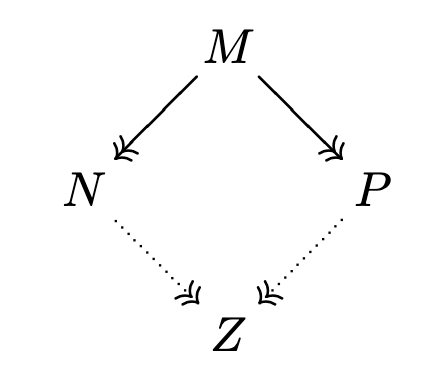
\includegraphics[width=0.2\textwidth]{figures/cr1.png}
    \caption{\textbf{Church-Rosser}定理的图示}\label{fig:church-rosser}
\end{figure}
\begin{corollary}
    如果$M=_\beta N$, 那么存在$Z\in \Lambda$, 使得$M\twoheadrightarrow Z$且$N\twoheadrightarrow Z$.
\end{corollary}
